\documentclass[a4paper,12pt]{article}
\usepackage[utf8]{inputenc}
\usepackage[T1]{fontenc}
\usepackage[english]{babel}
\usepackage{lmodern}
\usepackage{amsmath, amssymb, amsthm}
\usepackage{physics}
\usepackage{graphicx}
\usepackage{xcolor}
\usepackage{tikz}
\usepackage{setspace}
\usepackage{tcolorbox}
\usepackage{booktabs}
\usepackage{siunitx}
\usepackage{hyperref}
\usepackage{cleveref}
\usepackage{pgfplots}
\pgfplotsset{compat=1.18}
\usetikzlibrary{intersections}
\usepackage{tikz-feynman}

% Custom commands
\newcommand{\Tfield}{T(x)}
\newcommand{\DcovT}[1]{\Tfield D_\mu #1 + #1 \partial_\mu \Tfield}
\newcommand{\DhiggsT}{\Tfield (\partial_\mu + ig A_\mu) \Phi + \Phi \partial_\mu \Tfield}
\newcommand{\HiggsLagr}{\mathcal{L}_{\text{Higgs-T}}}
\newcommand{\FermionLagr}{\mathcal{L}_{\text{Fermion-T}}}
\newcommand{\BosonLagr}{\mathcal{L}_{\text{Boson-T}}}
\newcommand{\Mpl}{M_{\text{Pl}}}
\newcommand{\gammaf}{\gamma_{\text{Lorentz}}}

% Theorem styles
\newtheorem{theorem}{Theorem}[section]
\newtheorem{proposition}[theorem]{Proposition}
\newtheorem{corollary}[theorem]{Corollary}
\newtheorem{lemma}[theorem]{Lemma}
\theoremstyle{definition}
\newtheorem{definition}{Definition}
\theoremstyle{remark}
\newtheorem{remark}{Remark}
\usepackage{hyperref}

% Hyperref configuration
\hypersetup{
	colorlinks=true,
	linkcolor=blue,
	filecolor=magenta,
	urlcolor=blue,
	pdftitle={Time-Mass Duality: A Complementary Framework for Quantum Mechanics, Quantum Field Theory, and Cosmology},
	pdfauthor={Johann Pascher},
	pdfcreator={LaTeX}
}

% Repository base URL
\newcommand{\repobase}{https://github.com/jpascher/T0-Time-Mass-Duality/tree/main/2/}

\begin{document}
	
	\title{Time-Mass Duality: A Complementary Framework for Quantum Mechanics, Quantum Field Theory, and Cosmology}
	\author{Johann Pascher}
	\date{March 2025}
	\maketitle
	
	\begin{abstract}
		This paper presents the time-mass duality, a novel theoretical framework that extends the wave-particle duality by introducing a complementary dualism between time and mass. In the standard model, time varies (time dilation) while mass remains constant, whereas in the T0-model, time is absolute and mass varies as \( m = \frac{\hbar}{T c^2} \), where \( T(x) \) is a dynamic intrinsic time field. The intrinsic time, defined as \( T = \frac{\hbar}{m c^2} \), modifies the Schrödinger equation and quantum field theory (QFT), offering new interpretations of nonlocality, quantum gravity, and cosmological phenomena. Key parameters of the T0-model (\(\kappa\), \(\alpha\), \(\beta\)) are derived using natural units and perturbation theory, providing testable predictions. The framework explains flat rotation curves without dark matter, reinterprets dark energy as an energy exchange medium, and addresses the cosmological constant problem. Experimental tests, including mass-dependent Bell tests, cosmological observations, and CMB temperature measurements, are proposed to validate the model.
	\end{abstract}
	
	\tableofcontents
	\newpage
	
	\section{Introduction}
	
	Modern physics is built on dualistic concepts, such as the wave-particle duality, which describes how objects like electrons or photons exhibit both wave-like and particle-like properties[cite: 591, 592]. Similarly, quantum mechanics (QM) and quantum field theory (QFT) form a dualistic pair: QM emphasizes the discrete, particle-like nature of matter, while QFT focuses on continuous field concepts[cite: 593, 594]. However, both theories are incomplete:
	
	\begin{itemize}
		\item \textbf{Quantum Mechanics (QM)} describes quantum phenomena but struggles to fully incorporate relativistic effects[cite: 149, 150].
		\item \textbf{Quantum Field Theory (QFT)} unifies quantum effects with special relativity but faces challenges in integrating gravitation[cite: 149, 150].
	\end{itemize}
	
	Building on this inherent dualism, we introduce the time-mass duality, a new framework that proposes a complementary description of time and mass[cite: 596, 597]. In the standard model, time varies (time dilation) while mass remains constant, whereas in the T0-model, time is absolute and mass varies dynamically. This framework, developed in a series of works[cite: 596, 597], addresses fundamental issues in quantum mechanics, QFT, nonlocality, quantum gravity, and cosmology.
	
	\section{Theoretical Framework}
	
	\subsection{Wave-Particle Duality: A Precedent}
	
	The wave-particle duality is a cornerstone of quantum mechanics, describing how particles exhibit both wave-like and particle-like properties. Mathematically, these descriptions are connected via the Fourier transform:
	
	\begin{align}
		\Psi(\vec{x}) &= \frac{1}{(2\pi\hbar)^{3/2}} \int \phi(\vec{p}) e^{i\vec{p}\cdot\vec{x}/\hbar} d^3p, \\
		\phi(\vec{p}) &= \frac{1}{(2\pi\hbar)^{3/2}} \int \Psi(\vec{x}) e^{-i\vec{p}\cdot\vec{x}/\hbar} d^3x.
	\end{align}
	
	This duality highlights the complementary nature of position and momentum, governed by the uncertainty principle \( \Delta x \Delta p \geq \frac{\hbar}{2} \).
	
	\subsection{Time-Mass Duality: A New Complementary Framework}
	
	Analogous to the wave-particle duality, we propose a time-mass duality[cite: 596, 597]:
	
	\begin{itemize}
		\item \textbf{Time Dilation Description (Standard Model):} Time varies as \( t' = \gammaf t \), while rest mass remains constant[cite: 295, 296, 297, 298].
		\item \textbf{Mass Variation Description (T0-Model):} Time is absolute (\( T_0 = \text{const.} \)), while mass varies as \( m = \gammaf m_0 \), where \( \gammaf = \frac{1}{\sqrt{1 - v^2/c^2}} \)[cite: 298, 299, 300].
	\end{itemize}
	
	This duality is mathematically connected through a modified Lorentz transformation[cite: 598, 599]. The T0-model introduces the concept of intrinsic time, defined as:
	
	\begin{equation}
		T = \frac{\hbar}{m c^2},
	\end{equation}
	
	where \( T \) is a fundamental property of each object, dependent on its mass[cite: 300, 301, 302]. The intrinsic time leads to a modified Schrödinger equation:
	
	\begin{equation}
		i\hbar \frac{\partial}{\partial (t/T)} \Psi = \hat{H} \Psi,
	\end{equation}
	
	indicating that heavier objects experience faster internal time evolution than lighter ones[cite: 301, 302, 303, 304, 305].
	
	\subsection{Parallels Between Dualisms}
	
	The parallels between the wave-particle duality and the time-mass duality are significant[cite: 600, 601, 602]:
	
	\begin{enumerate}
		\item \textbf{Complementarity:} Just as position and momentum are complementary observables, time and energy/mass are complementary quantities.
		\item \textbf{Uncertainty Relations:} The wave-particle duality's \( \Delta x \Delta p \geq \frac{\hbar}{2} \) corresponds to \( \Delta t \Delta E \geq \frac{\hbar}{2} \) or \( \Delta T \Delta m \geq \frac{\hbar}{2 c^2} \) in the time-mass duality.
		\item \textbf{Transformations:} Both dualisms are connected through mathematical transformations.
	\end{enumerate}
	
	\section{Mathematical Formalism}
	
	\subsection{Lagrangian Formalism}
	
	The T0-model is formalized using a Lagrangian approach that incorporates the intrinsic time field \( \Tfield \)[cite: 648, 649]. The total Lagrangian density is:
	
	\begin{equation}
		\mathcal{L}_{\text{Total}} = \mathcal{L}_{\text{Boson}} + \mathcal{L}_{\text{Fermion}} + \mathcal{L}_{\text{Higgs-T}},
	\end{equation}
	
	with:
	
	\begin{align}
		\mathcal{L}_{\text{Boson}} &= -\frac{1}{4} \Tfield^2 F_{\mu\nu} F^{\mu\nu}, \\
		\mathcal{L}_{\text{Fermion}} &= \bar{\psi} i \gamma^\mu \DcovT{\psi} - y \bar{\psi} \Phi \psi, \\
		\mathcal{L}_{\text{Higgs-T}} &= (\DhiggsT)^\dagger (\DhiggsT) - \lambda (|\Phi|^2 - v^2)^2,
	\end{align}
	
	where \( \Tfield = \frac{\hbar}{y \langle \Phi \rangle c^2} \) is the intrinsic time field, linked to the Higgs vacuum expectation value[cite: 649, 650, 651].
	
	\subsection{Emergent Gravitation}
	
	Gravitation in the T0-model emerges from the gradients of the intrinsic time field[cite: 655, 656]:
	
	\begin{theorem}[Emergent Gravitation]
		Gravitation arises from the spatial and temporal gradients of the intrinsic time field:
		\begin{equation}
			\nabla \Tfield = -\frac{\hbar}{m^2 c^2} \nabla m \sim \nabla \Phi_g,
		\end{equation}
		where \( \Phi_g \) is the gravitational potential[cite: 655, 656].
	\end{theorem}
	
	\begin{proof}
		From \( \Tfield = \frac{\hbar}{m c^2} \), we derive:
		\begin{equation}
			\nabla \Tfield = -\frac{\hbar}{m^2 c^2} \nabla m.
		\end{equation}
		Using \( m(\vec{r}) = m_0 (1 + \frac{\Phi_g}{c^2}) \), we obtain:
		\begin{equation}
			\nabla m = \frac{m_0}{c^2} \nabla \Phi_g,
		\end{equation}
		and thus:
		\begin{equation}
			\nabla \Tfield \approx -\frac{\hbar}{m_0 c^4} \nabla \Phi_g.
		\end{equation}
	\end{proof}
	
	This emergent gravitation eliminates the need for a separate gravitational term in the Lagrangian, simplifying the theoretical framework[cite: 621, 622, 623].
	
	\subsection{Natural Units and Fundamental Constants}
	
	The T0-model employs natural units (\( \hbar = c = G = 1 \)) and sets the fine structure constant \( \alpha = 1 \) to simplify calculations[cite: 323, 324, 325]. This approach reinterprets physical constants as dimensionless ratios of energy, providing a unified perspective on fundamental constants[cite: 323, 324, 325]. Additionally, the Wien displacement constant \(\alpha_W \approx 2.82\) can be set to 1, redefining temperature as a frequency/energy unit[cite: 104, 105, 106, 107, 108].
	
	\section{Parameter Derivation}
	
	The T0-model introduces key parameters (\(\kappa\), \(\alpha\), \(\beta\)) that govern its predictions[cite: 213, 214, 215, 216, 217].
	
	\subsection{Derivation of \(\kappa\)}
	
	The parameter \(\kappa\) modifies the gravitational potential in the T0-model:
	
	\begin{equation}
		\Phi(r) = -\frac{G M}{r} + \kappa r.
	\end{equation}
	
	In natural units (\( \hbar = c = G = 1 \)):
	
	\begin{equation}
		\kappa = \beta \frac{y v}{r_g}, \quad r_g = \sqrt{\frac{M}{a_0}},
	\end{equation}
	
	where \( y \) is the Yukawa coupling, \( v \) is the Higgs vacuum expectation value, and \( a_0 \approx 1.2 \times 10^{-10} \, \text{m/s}^2 \) is a typical acceleration scale[cite: 195, 196, 197, 198]. In SI units:
	
	\begin{equation}
		\kappa_{\text{SI}} = \beta \frac{y v c^2}{r_g^2} \approx 4.8 \times 10^{-11} \, \text{m/s}^2.
	\end{equation}
	
	\subsection{Derivation of \(\alpha\)}
	
	The parameter \(\alpha\) describes the photon energy loss rate, leading to cosmological redshift:
	
	\begin{equation}
		1 + z = e^{\alpha r}.
	\end{equation}
	
	In natural units:
	
	\begin{equation}
		\alpha = \frac{\lambda_h^2 v}{L_T}, \quad L_T \sim \frac{\Mpl}{m_h^2 v},
	\end{equation}
	
	where \( \lambda_h \) is the Higgs wavelength, \( m_h \) is the Higgs mass, and \( L_T \) is the correlation length. In SI units:
	
	\begin{equation}
		\alpha_{\text{SI}} = \frac{\lambda_h^2 v c^2}{L_T} \approx 2.3 \times 10^{-18} \, \text{m}^{-1}.
	\end{equation}
	
	The correlation length \( L_T \) is derived from Higgs fluctuations:
	
	\begin{equation}
		L_T \sim \frac{\Mpl}{m_h^2 v} \approx 6.3 \times 10^{27} \, \text{m}.
	\end{equation}
	
	\subsection{Derivation of \(\beta\)}
	
	The parameter \(\beta\) governs the wavelength-dependent redshift:
	
	\begin{equation}
		z(\lambda) = z_0 \left(1 + \beta \ln \frac{\lambda}{\lambda_0}\right).
	\end{equation}
	
	In natural units:
	
	\begin{equation}
		\beta = \frac{\lambda_h^2 v^2}{4 \pi^2 \lambda_0 \alpha_0}.
	\end{equation}
	
	Using perturbation theory and Feynman diagrams, we obtain:
	
	\begin{equation}
		\beta = \frac{(2\pi)^4 m_h^2}{16 \pi^2 v^4 y^2 \Mpl^2 \lambda_0^4 \alpha_0} \approx 0.008.
	\end{equation}
	
	The Feynman diagram for this interaction involves photon-Higgs scattering:
	
	\begin{center}
		\feynmandiagram [horizontal=a to b] {
			a [particle=\(\gamma\)] -- [photon] b -- [photon] f [particle=\(\gamma\)],
			b -- [scalar, half left] c -- [scalar, half left] b,
			c -- [photon] d,
		};
	\end{center}
	
	\section{Extensions to Quantum Mechanics and Quantum Field Theory}
	
	\subsection{Extension of Quantum Mechanics}
	
	The classical Schrödinger equation is modified to account for intrinsic time[cite: 395, 396, 397]:
	
	\begin{equation}
		i\hbar \frac{\partial}{\partial (t/T)} \Psi = \hat{H} \Psi,
	\end{equation}
	
	where \( T = \frac{\hbar}{m c^2} \). This modification leads to:
	
	\begin{itemize}
		\item Mass-dependent time evolution of quantum systems.
		\item A natural explanation for different decay rates and coherence times, with decoherence rate:
		\begin{equation}
			\Gamma_{\text{dec}} = \Gamma_0 \cdot \frac{m c^2}{\hbar}.
		\end{equation}
		\item A new perspective on the measurement problem through the connection between mass and time evolution[cite: 146, 147, 148, 149].
	\end{itemize}
	
	\subsection{Extension of Quantum Field Theory}
	
	QFT is extended to incorporate absolute time or mass-dependent intrinsic time[cite: 514, 515, 516, 517]:
	
	\begin{itemize}
		\item Field operators are reformulated in terms of intrinsic time \( T = \frac{\hbar}{m c^2} \).
		\item Renormalization is reinterpreted through mass-dependent time scales.
		\item Virtual particles are understood as manifestations of different intrinsic time scales.
	\end{itemize}
	
	These extensions are particularly promising for:
	
	\begin{itemize}
		\item Integrating gravitation into QFT.
		\item Resolving infinities in QFT.
		\item Understanding vacuum energy and the cosmological constant problem[cite: 285, 286, 287].
	\end{itemize}
	
	\section{Dynamic Mass of Photons and Nonlocality}
	
	\subsection{Dynamic Mass of Photons}
	
	In the T0-model, photons are assigned a dynamic, frequency-dependent mass[cite: 162, 163, 164]:
	
	\begin{equation}
		m_\gamma = \omega,
	\end{equation}
	
	where \(\omega\) is the angular frequency of the photon. The intrinsic time for photons is defined as:
	
	\begin{equation}
		T = \frac{1}{E},
	\end{equation}
	
	where \( E \) is the photon energy. A unified model combines the T0-model with intrinsic time:
	
	\begin{equation}
		T = \frac{1}{\max(m, E)},
	\end{equation}
	
	ensuring consistency across particles and photons[cite: 167, 168, 169].
	
	\subsection{Implications for Nonlocality}
	
	The dynamic mass of photons affects quantum nonlocality, particularly in entangled systems[cite: 342, 343, 344, 345, 346]. In the standard model, nonlocality is often interpreted as instantaneous action at a distance, which appears to conflict with relativity. The T0-model provides an alternative:
	
	\begin{itemize}
		\item In the T0-model with absolute time, quantum correlations arise from mass variation (\( m = \gamma m_0 \)) rather than temporal effects.
		\item In the intrinsic time model, entangled particles with different masses experience different time evolutions. A lighter particle with larger \( T \) reacts more slowly to state changes than a heavier particle with smaller \( T \)[cite: 308, 309, 310, 311, 312, 313, 314, 315].
		\item For photons, intrinsic time is defined as \( T = \frac{1}{E} \), corresponding to the wavelength. A higher-energy (shorter-wavelength) photon experiences faster time evolution than a lower-energy photon.
	\end{itemize}
	
	This perspective replaces the counterintuitive notion of instantaneous action with a systematic, mass-dependent dynamics, which could be empirically tested through Bell tests with particles of different masses or photons of different frequencies[cite: 387, 388, 389, 390, 391, 392, 393, 394]. The energy-dependent correlation delay is:
	
	\begin{equation}
		\Delta t \propto \left| \frac{1}{E_1} - \frac{1}{E_2} \right|.
	\end{equation}
	
	\begin{figure}[h]
		\centering
		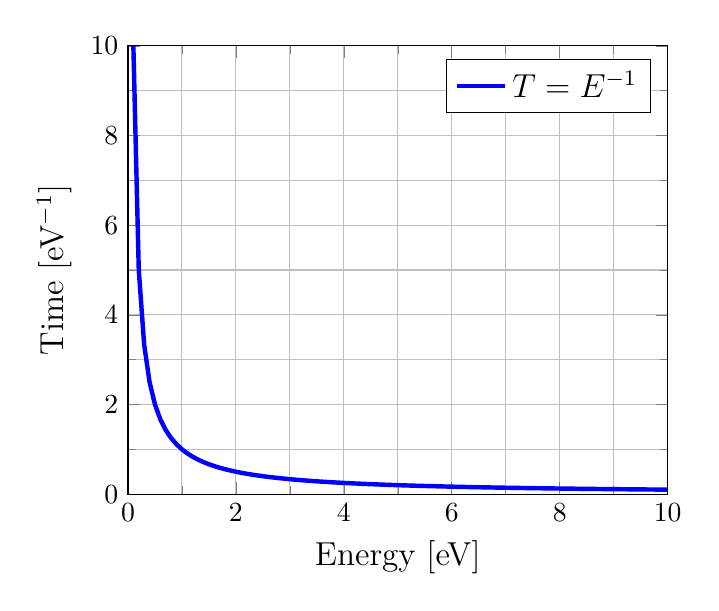
\begin{tikzpicture}
			\begin{axis}[
				xlabel={Energy [eV]},
				ylabel={Time [eV\(^{-1}\)]},
				xlabel style={font=\large},
				ylabel style={font=\large},
				tick label style={font=\normalsize},
				xmin=0, xmax=10,
				ymin=0, ymax=10,
				legend pos=north east,
				legend style={font=\large},
				grid=both,
				minor tick num=1
				]
				\addplot[blue, ultra thick, domain=0.1:10, samples=100] {1/x};
				\legend{\(T = E^{-1}\)}
			\end{axis}
		\end{tikzpicture}
		\caption{Energy-dependent time for photons in the T0-model, illustrating the inverse relationship between photon energy and intrinsic time.}
		\label{fig:energy_time_photons}
	\end{figure}
	
	\section{Results and Implications}
	
	\subsection{Nonlocality and Quantum Correlations}
	
	The time-mass duality offers a new interpretation of nonlocality in quantum physics[cite: 346, 347, 348, 349, 350, 351]. The mass-dependent time evolution leads to measurable delays in quantum correlations, providing a deterministic framework for understanding entanglement without invoking instantaneous action at a distance.
	
	\subsection{Cosmological Implications}
	
	The T0-model has significant implications for cosmology[cite: 173, 174, 175, 176, 177]:
	
	\begin{itemize}
		\item \textbf{Flat Rotation Curves:} The model explains flat rotation curves without dark matter through a modified gravitational potential \( \Phi(r) = -\frac{G M}{r} + \kappa r \), where \( \kappa \approx 4.8 \times 10^{-11} \, \text{m/s}^2 \)[cite: 624, 625, 626, 627, 628, 629, 630].
		\item \textbf{Dark Energy Reinterpretation:} Dark energy is reinterpreted as a mechanism for energy distribution rather than the cause of cosmic expansion[cite: 178, 179, 180, 181, 182, 183, 184].
		\item \textbf{CMB Interpretation:} The model predicts a larger angular diameter distance at the CMB (\( z = 1100 \)), leading to an angular size of structures of \( 5.8^\circ \) compared to \( 1^\circ \) in the \( \Lambda \)CDM model[cite: 45, 46, 47, 48, 49, 50, 51, 52, 53, 54, 55, 56].
	\end{itemize}
	
	\subsection{Dark Energy as an Energy Exchange Medium}
	
	In the T0-model, dark energy is modeled as a dynamic scalar field \(\phi_{DE}\) that facilitates energy exchange in a static universe[cite: 185, 186, 187]. The Lagrangian density for the dark energy field is:
	
	\begin{equation}
		\mathcal{L}_{DE} = -\frac{1}{2} \partial_\mu \phi_{DE} \partial^\mu \phi_{DE} - V(\phi_{DE}) - \frac{\beta}{M_{Pl}} \phi_{DE} T^{\mu}_{\mu} - \frac{1}{2} \xi \phi_{DE}^2 R,
	\end{equation}
	
	where \( V(\phi_{DE}) = \frac{1}{2} m_\phi^2 \phi_{DE}^2 + \lambda \phi_{DE}^4 \). The field equation simplifies for a massless field (\( m_\phi \approx 0 \)) and negligible curvature (\( \xi R \approx 0 \)):
	
	\begin{equation}
		\frac{1}{r^2} \frac{d}{dr} \left(r^2 \frac{d\phi_{DE}}{dr}\right) = 4 \lambda \phi_{DE}^3 + \frac{\beta}{M_{Pl}} T^{\mu}_{\mu}.
	\end{equation}
	
	This leads to an energy density profile of:
	
	\begin{equation}
		\rho_{DE}(r) \approx \frac{\kappa}{r^2},
	\end{equation}
	
	consistent with observations[cite: 188, 189, 190, 191].
	
	\section{Discussion}
	
	The time-mass duality offers a novel perspective that unifies various aspects of physics. By reinterpreting time and mass, it provides new insights into quantum mechanics, QFT, and cosmology. The model's predictions, such as mass-dependent delays in entanglement and alternative explanations for dark energy, are testable and could lead to a deeper understanding of the universe.
	
	\section{Conclusion}
	
	The time-mass duality presents a complementary framework to the wave-particle duality, offering a fresh perspective on fundamental physics. It addresses key challenges in modern physics, from nonlocality to the cosmological constant problem, and opens avenues for future research and experimental verification.
	
	\begin{thebibliography}{99}
		\bibitem{bohr1928} Bohr, N. (1928). The Quantum Postulate and the Recent Development of Atomic Theory. \textit{Nature}, 121(3050), 580-590.
		\bibitem{weinberg1995} Weinberg, S. (1995). \textit{The Quantum Theory of Fields, Volume 1: Foundations}. Cambridge University Press.
		\bibitem{dirac1928} Dirac, P. A. M. (1928). The Quantum Theory of the Electron. \textit{Proceedings of the Royal Society of London. Series A, Containing Papers of a Mathematical or Physical Character}, 117(778), 610-624.
		\bibitem{witten2001} Witten, E. (2001). Quantum Gravity. In \textit{Encyclopedia of Physical Science and Technology} (3rd ed., Vol. 13, pp. 1-13). Academic Press.
		\bibitem{pascher_kompl_2025} Pascher, J. (2025). Complementary Extensions of Physics: Absolute Time and Intrinsic Time.
		\bibitem{pascher_kurzgefasst_2025} Pascher, J. (2025). Abstract - Complementary Dualism in Physics: From Wave-Particle to Time-Mass Concepts.
		\bibitem{pascher_zeit_2025} Pascher, J. (2025). Time as an Emergent Property in Quantum Mechanics: A Connection Between Relativity, Fine Structure Constant, and Quantum Dynamics.
		\bibitem{pascher_math_2025} Pascher, J. (2025). Mathematical Formulation of the Higgs Mechanism in Time-Mass Duality.
		\bibitem{pascher_wesentl_2025} Pascher, J. (2025). Essential Mathematical Formalisms of the Time-Mass Duality Theory with Lagrangian Densities.
		\bibitem{pascher_verein_2025} Pascher, J. (2025). Unification of the T0-Model: Foundations, Dark Energy, and Galactic Dynamics.
		\bibitem{pascher_messdifferenzen_2025} Pascher, J. (2025). Compensatory and Additive Effects: An Analysis of Measurement Differences between the T0 Model and the $\Lambda$CDM Standard Model.
		\bibitem{pascher_notwendigkeit_2025} Pascher, J. (2025). The Necessity of Extending Standard Quantum Mechanics and Quantum Field Theory.
		\bibitem{pascher_parameter_2025} Pascher, J. (2025). Parameter Derivation in the T0-Model.
		\bibitem{pascher_energiedynamik_2025} Pascher, J. (2025). Dark Energy in the T0 Model: A Mathematical Analysis of Energy Dynamics.
		\bibitem{pascher_dynamische_masse_2025} Pascher, J. (2025). Dynamic Mass of Photons and Its Implications for Nonlocality.
		\bibitem{pascher_perspective_2025} Pascher, J. (2025). A New Perspective on Time and Space: Johann Pascher’s Revolutionary Ideas.
		\bibitem{pascher_temperature_2025} Pascher, J. (2025). Adjustment of Temperature Units in Natural Units and CMB Measurements.
		\bibitem{pascher_massenvariation_2025} Pascher, J. (2025). Mass Variation in Galaxies: An Analysis in the T0-Model with Emergent Gravitation.
		\bibitem{pascher_jenseits_2025} Pascher, J. (2025). Real Consequences of the Reformulation of Time and Mass in Physics: Beyond the Planck Scale.
		\bibitem{pascher_natuerliche_einheiten_2025} Pascher, J. (2025). Fundamental Constants and Their Derivation from Natural Units.
	\end{thebibliography}
	
\end{document}